  \documentclass[../Report.tex]{subfiles}

\begin{document}

\chapter{Implementation and Testing} \label{chap:imp_test}

\section{Implementation of AI model}

\subsection{Dataset}
Any AI models need datasets, so the following are datasets:
\begin{description}
  \item[Crop Prediction:] Dataset for crop prediction is obtained by web scrapping google images. These images aren't perfect, so every image
  is manually checked if its correct and is not blurry, or has other elements.

  \item[Disease Detection: ] Dataset of Crop Disease Detection is a combination of two different datasets.
  \begin{itemize}
    \item First, is Plant Village Dataset\cite{disease_dataset} which contains 54,306 images of 14 crop species and 26 diseases. This is a 
    dataset of plant leaves colleted in labs.

    \item Second, is a PlantDoc Dataset\cite{plactdoc} which contains 2,598 images in total across 13 plant species and up to 17 classes 
    of diseases. These images are collected in field and have a little more noise and are closer to real-world images.
  \end{itemize}
\end{description}

\subsection{Model Architecture}
Convolutional Neural Network (CNN or ConvNet) \cite{cnn} is a class of deep neural networks, most commonly applied to analyzing visual imagery.
They are also known as shift invariant or space invariant artificial neural networks (SIANN), based on their shared-weights architecture and 
translation invariance characteristics.\par

CNNs makes it easy to perform Image Classification by sharing weights, this means CNNs use less memory compared to simple Artificial Neural 
Networks with same perform. But, CNNs still take a long time to train, so instead of trying to create a CNN from the bottom-up, we can use 
transfer learning to use a pre-trained ConvNet.\par

In this project, we use ResNet that has been pre-trained on ImageNet \cite{imagenet}. ImageNet is a large visual dataset containing more than 
14 million images with over 20,000 categories. This gives us a huge advantage as the ConvNet has essentially learned the basics of vision, 
like detecting edges, lines, shapes, etc.\par

\subsection{Data Pre-processing}
\begin{description}
  \item[Crop Prediction:] Before passing image to ConvNet, they need to be slightly processed. This depends if we are training or 
  testing/inference. During training, images are randomly cropped to size $320px \times 320px$, flipped and normalized. 
  During testing/inference, images are resized to $480px \times 480px$, then center cropped to size $320px \times 320px$ and normalized.

  \begin{lstlisting}[language=python,caption={Crop Prediction Image Pre-processing},captionpos=b]
    data_transforms = {
      "train": transforms.Compose([
        transforms.RandomResizedCrop(320),
        transforms.RandomHorizontalFlip(),
        transforms.ToTensor(),
        transforms.Normalize([0.485, 0.456, 0.406], [0.229, 0.224, 0.225])
      ]),
      
      "val": transforms.Compose([
        transforms.Resize(480),
        transforms.CenterCrop(320),
        transforms.ToTensor(),
        transforms.Normalize([0.485, 0.456, 0.406], [0.229, 0.224, 0.225])
      ])
    }
  \end{lstlisting}

  \item[Disease Detection]: Pre-processing for disease detection is similar to crop prediction with slight differences.
  
  \begin{lstlisting}[language=python,caption={Disease Detection Image Pre-processing},captionpos=b]
    data_transforms = {
      'train': transforms.Compose([
        transforms.RandomRotation(30),
        transforms.RandomResizedCrop(224),
        transforms.RandomHorizontalFlip(),
        transforms.ToTensor(),
        transforms.Normalize([0.485, 0.456, 0.406], [0.229, 0.224, 0.225])
      ]),
      'valid': transforms.Compose([
        transforms.Resize(256),
        transforms.CenterCrop(224),
        transforms.ToTensor(),
        transforms.Normalize([0.485, 0.456, 0.406], [0.229, 0.224, 0.225])
      ]),
    }
  \end{lstlisting}

\end{description}

\subsection{Defining Model}

As specified, we are using transfer learning technique, for crop detection, we use ResNet50 and for disease detection, we use ResNet152.
We are not training the entire ResNet, so we simply remove the last layer of ResNet and replace with new layer(s) and freeze the other 
layers to prevent training of those layers.

The following is the code snippets for loading the model
\begin{lstlisting}[language=python,caption={Defining Model},captionpos=b]
  model = models.resnet50(pretrained=True) # model = models.resnet152(pretrained=True) (for disease detection)
  for param in model.parameters():
  param.requires_grad = False

  fc_in_ftrs = model.fc.in_features
  fc_out_ftrs = len(class_names)
  model.fc = nn.Sequential(nn.Linear(fc_in_ftrs, 1024),
                        nn.ReLU(),
                        nn.Dropout(0.2),
                        nn.Linear(1024, fc_out_ftrs))
\end{lstlisting}

\subsection{Defining Cost, Optimization Function and Training Model}

\begin{description}
  \item[Crop Prediction:] We are using Stochastic Gradient Descent (SGD) with momentum as optimization algorithm and CrossEntropyLoss as 
  Loss function. The model is trained for 50 epochs with a batch size of 16 with learning rate decay rate $\gamma$ of 0.1 for every 10 epochs.

  \begin{lstlisting}[language=python,caption={Disease Detection Image Pre-processing},captionpos=b]
    criterion = nn.CrossEntropyLoss()
    optimizer = optim.SGD(model.fc.parameters(), lr=0.001, momentum=0.9)
    exp_mr_scheduler = lr_scheduler.StepLR(optimizer, step_size=10, gamma=0.1)
    model, best_acc = train_model(model, criterion, optimizer, exp_mr_scheduler, num_epochs=50)
  \end{lstlisting}

  \begin{figure}[H]
    \centering
    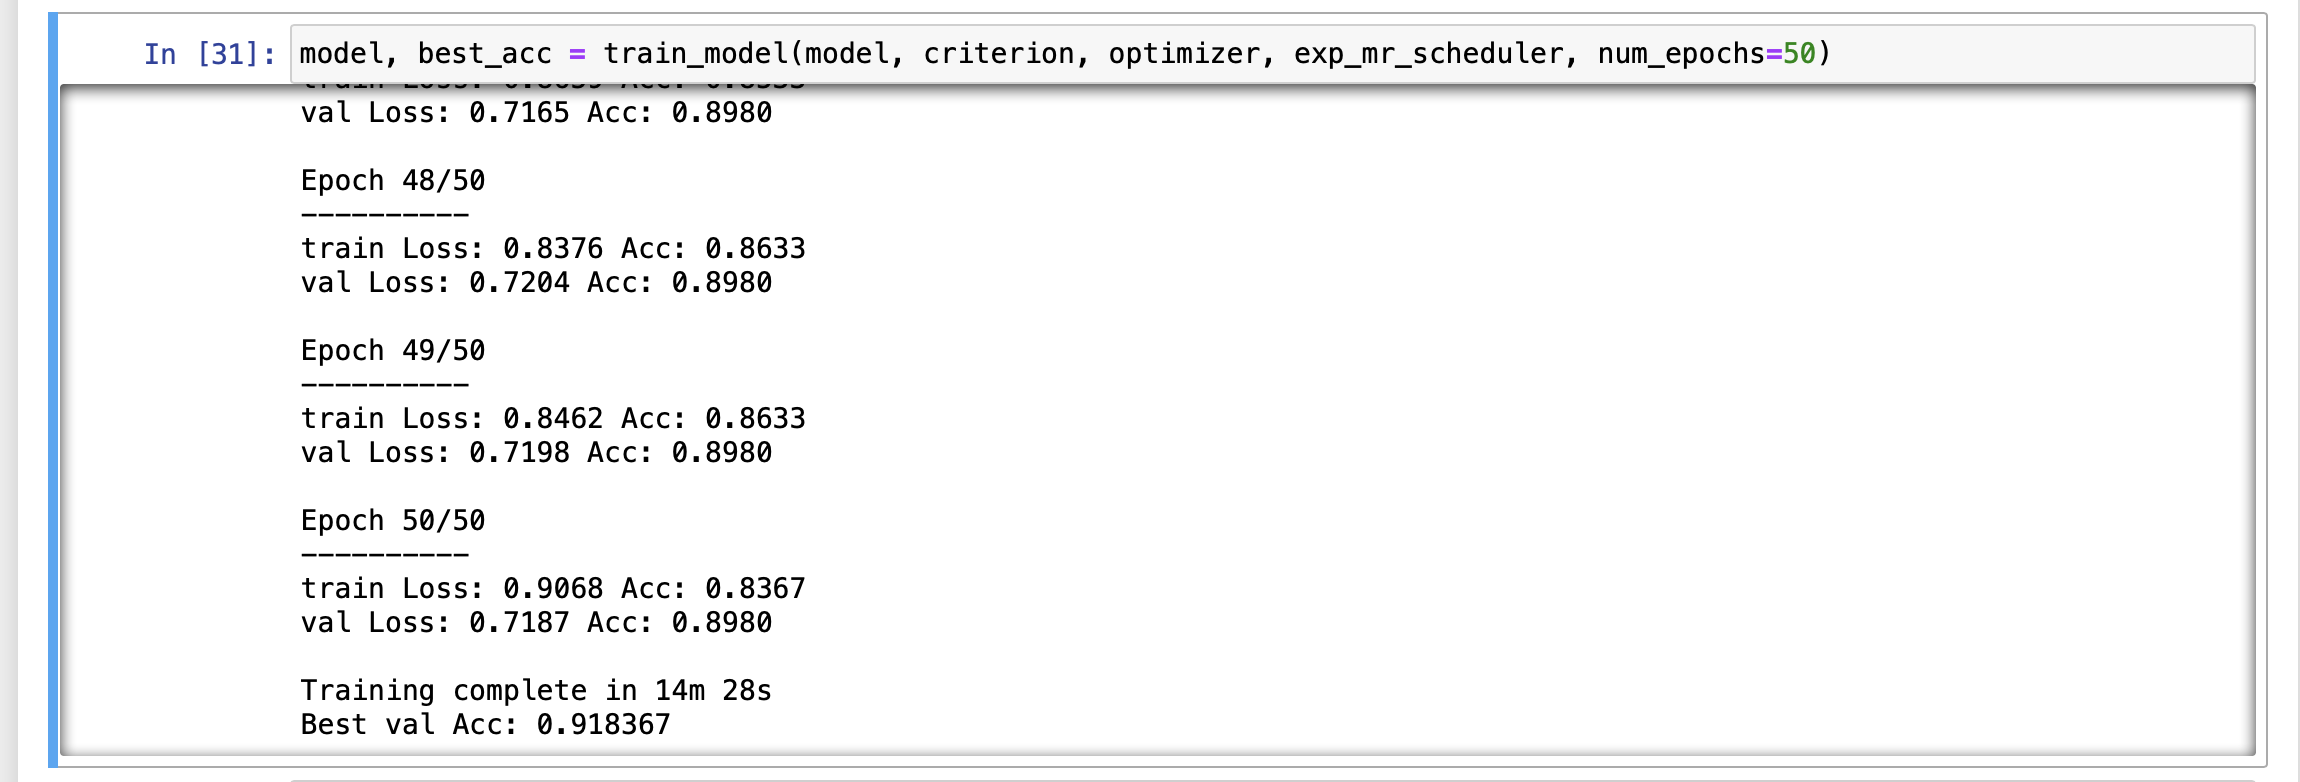
\includegraphics[width=\linewidth]{images/crop_acc.png}
    \caption{Crop Detection Accuracy}
    \label{fig:crop_acc}
  \end{figure}

  \item[Disease Detection:] We are using \cite{adam} Optimizer and Negative Log Likelihood (NLLLoss) as Loss function. The model is trained for 
  10 epochs with a batch size of 16 with learning rate decay rate $\gamma$ of 0.1 for every 5 epochs.
  \begin{lstlisting}[language=python,caption={Disease Detection Image Pre-processing},captionpos=b]
    criterion = nn.NLLLoss()
    optimizer = optim.Adam(model.fc.parameters(), lr=0.001)
    exp_lr_scheduler = lr_scheduler.StepLR(optimizer, step_size=5, gamma=0.1)
    
    model, best_acc = train_model(model, criterion, optimizer, exp_lr_scheduler, num_epochs=10) 
  \end{lstlisting}

  \begin{figure}[H]
    \centering
    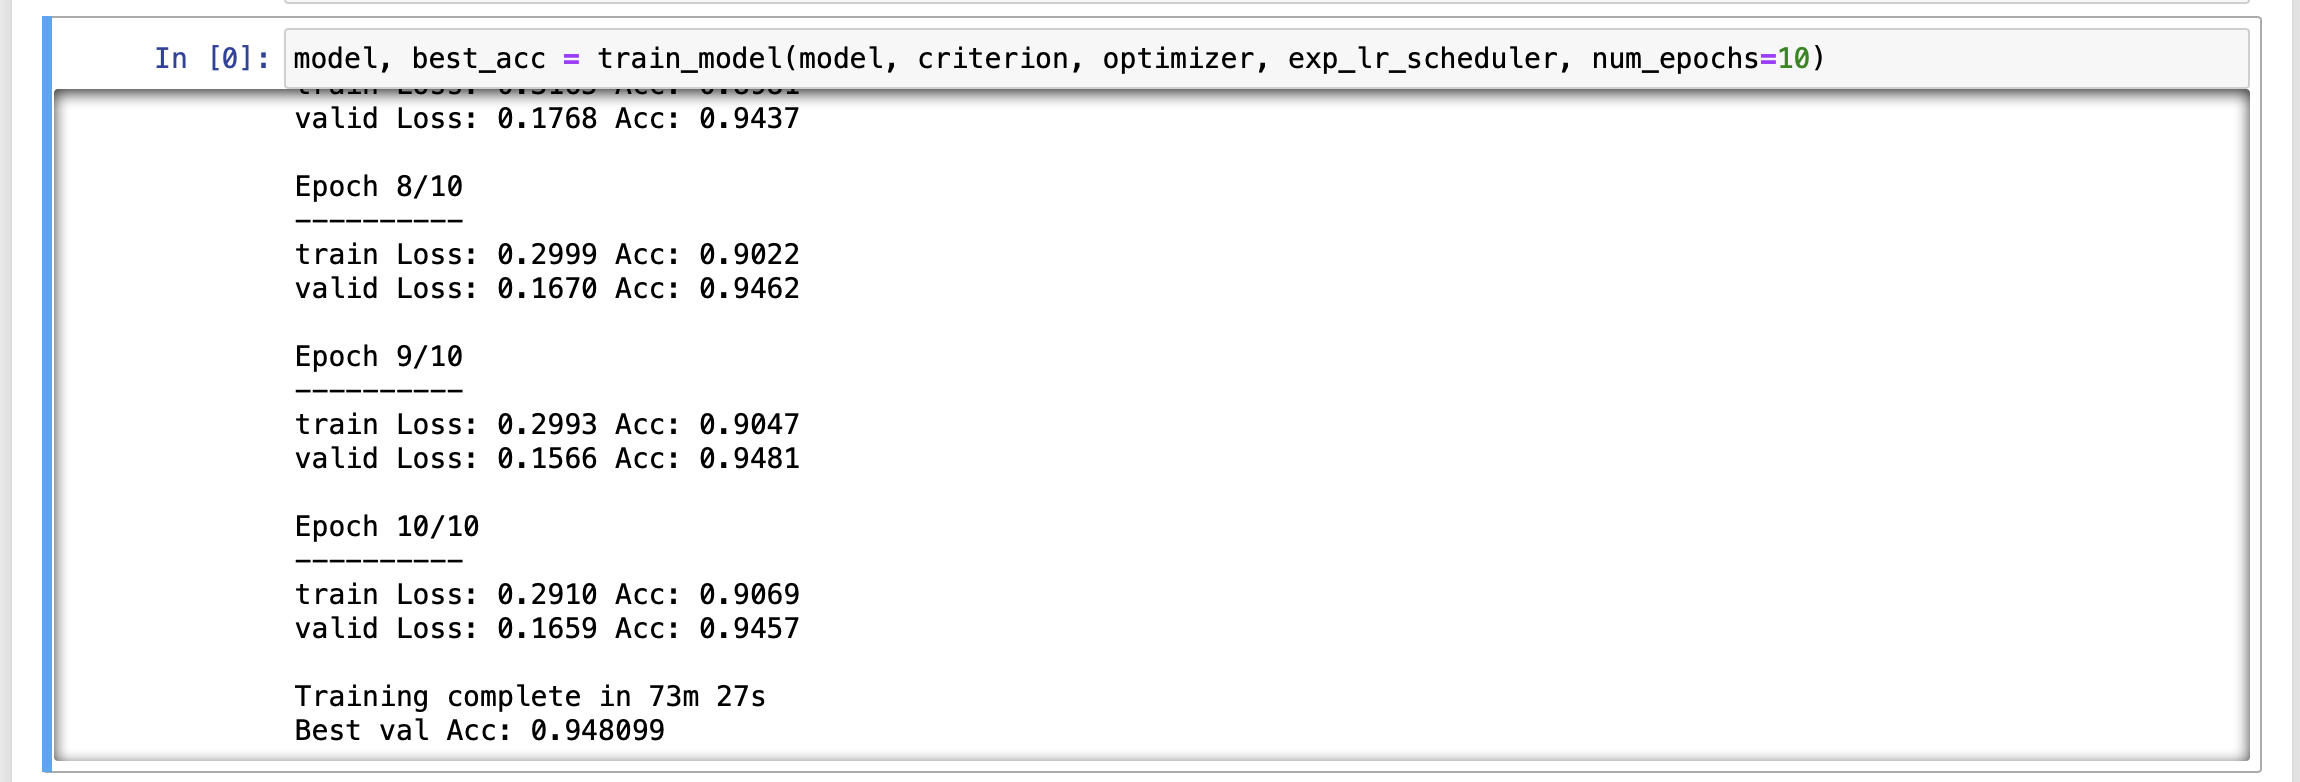
\includegraphics[width=\linewidth]{images/disease_acc.png}
    \caption{Crop Detection Accuracy}
    \label{fig:disease_acc}s
  \end{figure}

\end{description}

\section{Implementation of Inference Server} \label{sec:inference_server}

Inference Server is implemented using flask to make is simple ad light-weight. This is a very simple server, it just has to endpoints.

\begin{itemize}
  \item \texttt{http://<server\_ip>/crop}
  \item \texttt{http://<server\_ip>/disease}
\end{itemize}

When any one of these endpoints, receives a request, bytes of data are converted to image, pre-processing is applied appropriately 
and send to the respect AI model. Following is a snippet of the inference code.

\begin{lstlisting}[language=python,caption={Crop Inference Code},captionpos=b]
  def get_crop_prediction(image_bytes):
    tensor = crop_transform_image(image_bytes)
    outputs = crop_model.forward(tensor).squeeze(0)
    _, pred = outputs.max(0)
    outputs = F.softmax(outputs, dim=0)
    preds = [float(f"{outputs[i].item():.4f}") for i in range(len(crop_class_names))]
    return {"pred": pred.item(), "cnf": preds, "kind": "crop"}
\end{lstlisting}

\begin{lstlisting}[language=python,caption={Crop Inference Code},captionpos=b]
  def get_disease_prediction(image_bytes):
    tensor = disease_transform_image(image_bytes)
    outputs = disease_model.forward(tensor).squeeze(0)
    _, pred = outputs.max(0)
    preds = [float(f"{outputs[i].item():.4f}") for i in range(len(diseases_class_names))]
    return {"pred": pred.item(), "cnf": preds, "kind": "disease"}
\end{lstlisting}

The returned value is a dictionary, this is converted to JSON and send back to the mobile app.

\section{Connection between Mobile App and Inference Server}

REST APIs are used for communication between Mobile App and Inference Server. But this communication cannot be done using only JSON.
Image are too large to be sent using JSON, so multipart/form-data request is used, to send images to server as bytes. At the server-side,
the images are converted from bytes and passed to AI model as shown above in section. \ref{sec:inference_server}.\par

Both iOS and Android have different Implementations for preforming multipart/form-data. In android, a custom Volley\cite{volloy} request 
is used and in iOS, default URLSession can be used for multipart/form-data request.\par

\noindent \textbf{iOS Implementation:}

\begin{lstlisting}[language=swift,caption={iOS multipart/form-data request Implementation},captionpos=b]
  let filename = "cropimage.png"
  let boundary = UUID().uuidString
        
  var request = URLRequest(url: URLs[kind]!)
  request.httpMethod = "POST"
  request.setValue("multipart/form-data; boundary=\(boundary)", forHTTPHeaderField: "Content-Type")
        
  var data = Data()
        
  data.append("\r\n--\(boundary)\r\n".data(using: .utf8)!)
  data.append("Content-Disposition: form-data; name=\"img\"; filename=\"\(filename)\"\r\n".data(using: .utf8)!)
  data.append("Content-Type: image/png\r\n\r\n".data(using: .utf8)!)
  data.append(image.pngData()!)
  data.append("\r\n--\(boundary)--\r\n".data(using: .utf8)!)
        
  URLSession.shared.uploadTask(with: request, from: data) { data, response, error in
    guard let data = data else {
      // An error occurred
      print(error?.localizedDescription ?? "Unknown Error")
      completionHandler(nil)
      return
    }
    
    // Response received, JSON is converted to an Swift Object
    let prediction = try? JSONDecoder().decode(Prediction.self, from: data)
    prediction?.image = image
    completionHandler(prediction)
  }.resume()
\end{lstlisting}

\noindent \textbf{Android Implementation:}
\begin{lstlisting}[language=java,caption={Android multipart/form-data request Implementation},captionpos=b]
  ByteArrayOutputStream outputStream = new ByteArrayOutputStream();
  bitmap.compress(Bitmap.CompressFormat.PNG, 100, outputStream);
  final byte[] imageBytes = outputStream.toByteArray();

  String url = getURL(context, kind);
  VolleyMultipartRequest request = new VolleyMultipartRequest(Request.Method.POST, url,
      new Response.Listener<NetworkResponse>() {
        @Override
        public void onResponse(NetworkResponse response) {
          Gson gson = new GsonBuilder()
                  .registerTypeAdapter(Prediction.class, new PredictionDeserializer())
                  .create();

          Prediction prediction = gson.fromJson(new String(response.data), Prediction.class);
          prediction.image = bitmap;
          callback.onCropPrediction(prediction);
        }
      },
      new Response.ErrorListener() {
        @Override
        public void onErrorResponse(VolleyError volleyError) {
          volleyError.printStackTrace();
          callback.onCropPrediction(null);
        }
      }) {
      @Override
      protected Map<String, String> getParams() {
        Map<String, String> params = new HashMap<>();
        return params;
      }

      @Override
      protected Map<String, DataPart> getByteData() {
        Map<String, DataPart> params = new HashMap<>();
        params.put("img", new DataPart("crop.jpg", imageBytes));

        return params;
      }
    };

    VolleySingleton.getInstance(context).addToRequestQueue(request);
\end{lstlisting}

This is a partial implementation. The full implementation is very lengthy, please refer Volloy Docs for more details.

\section{Implementation of Mobile App}

We developed native Android and iOS mobile apps with user the same Inference server and data models. This means the user can use any platform
and all of the user's data is automatically synced between devices.

\begin{itemize}
  \item Frequently accessed data from database is cached locally to speed up the process.
  \item All network requests are asynchronous, so that the app is always responsive
  \item State Observers are used to observer any changes in data and update the UI accordingly.
  \item All images are cached to prevent constant retrieval from the cloud.
\end{itemize}

\noindent
GitHub Repos
\begin{description}
  \item [iOS App:] $\texttt{https://github.com/SaiHemanthBR/CropPrediction-ios}$
  \item[Android App:] $\texttt{https://github.com/SaiHemanthBR/CropPrediction-Android}$
\end{description}

\section{Testing}

Testing is done both manually and automatically. Manual testing involves running the app and checking if all the features are working as 
intended.\par
Automated testing involves writing test cases that evaluate the functionality of app as small individual parts and later after integration 
as a whole.

\subsection{AI model accuracy validation} \label{sec:ai_testing}

For both crop detection and disease detection, a subset of images from the dataset is made into test dataset. This test dataset is used to 
test the accuracy of AI model.\par

Crop Detection AI model has an accuracy of 91.8\%.
\begin{figure}[H]
  \centering
  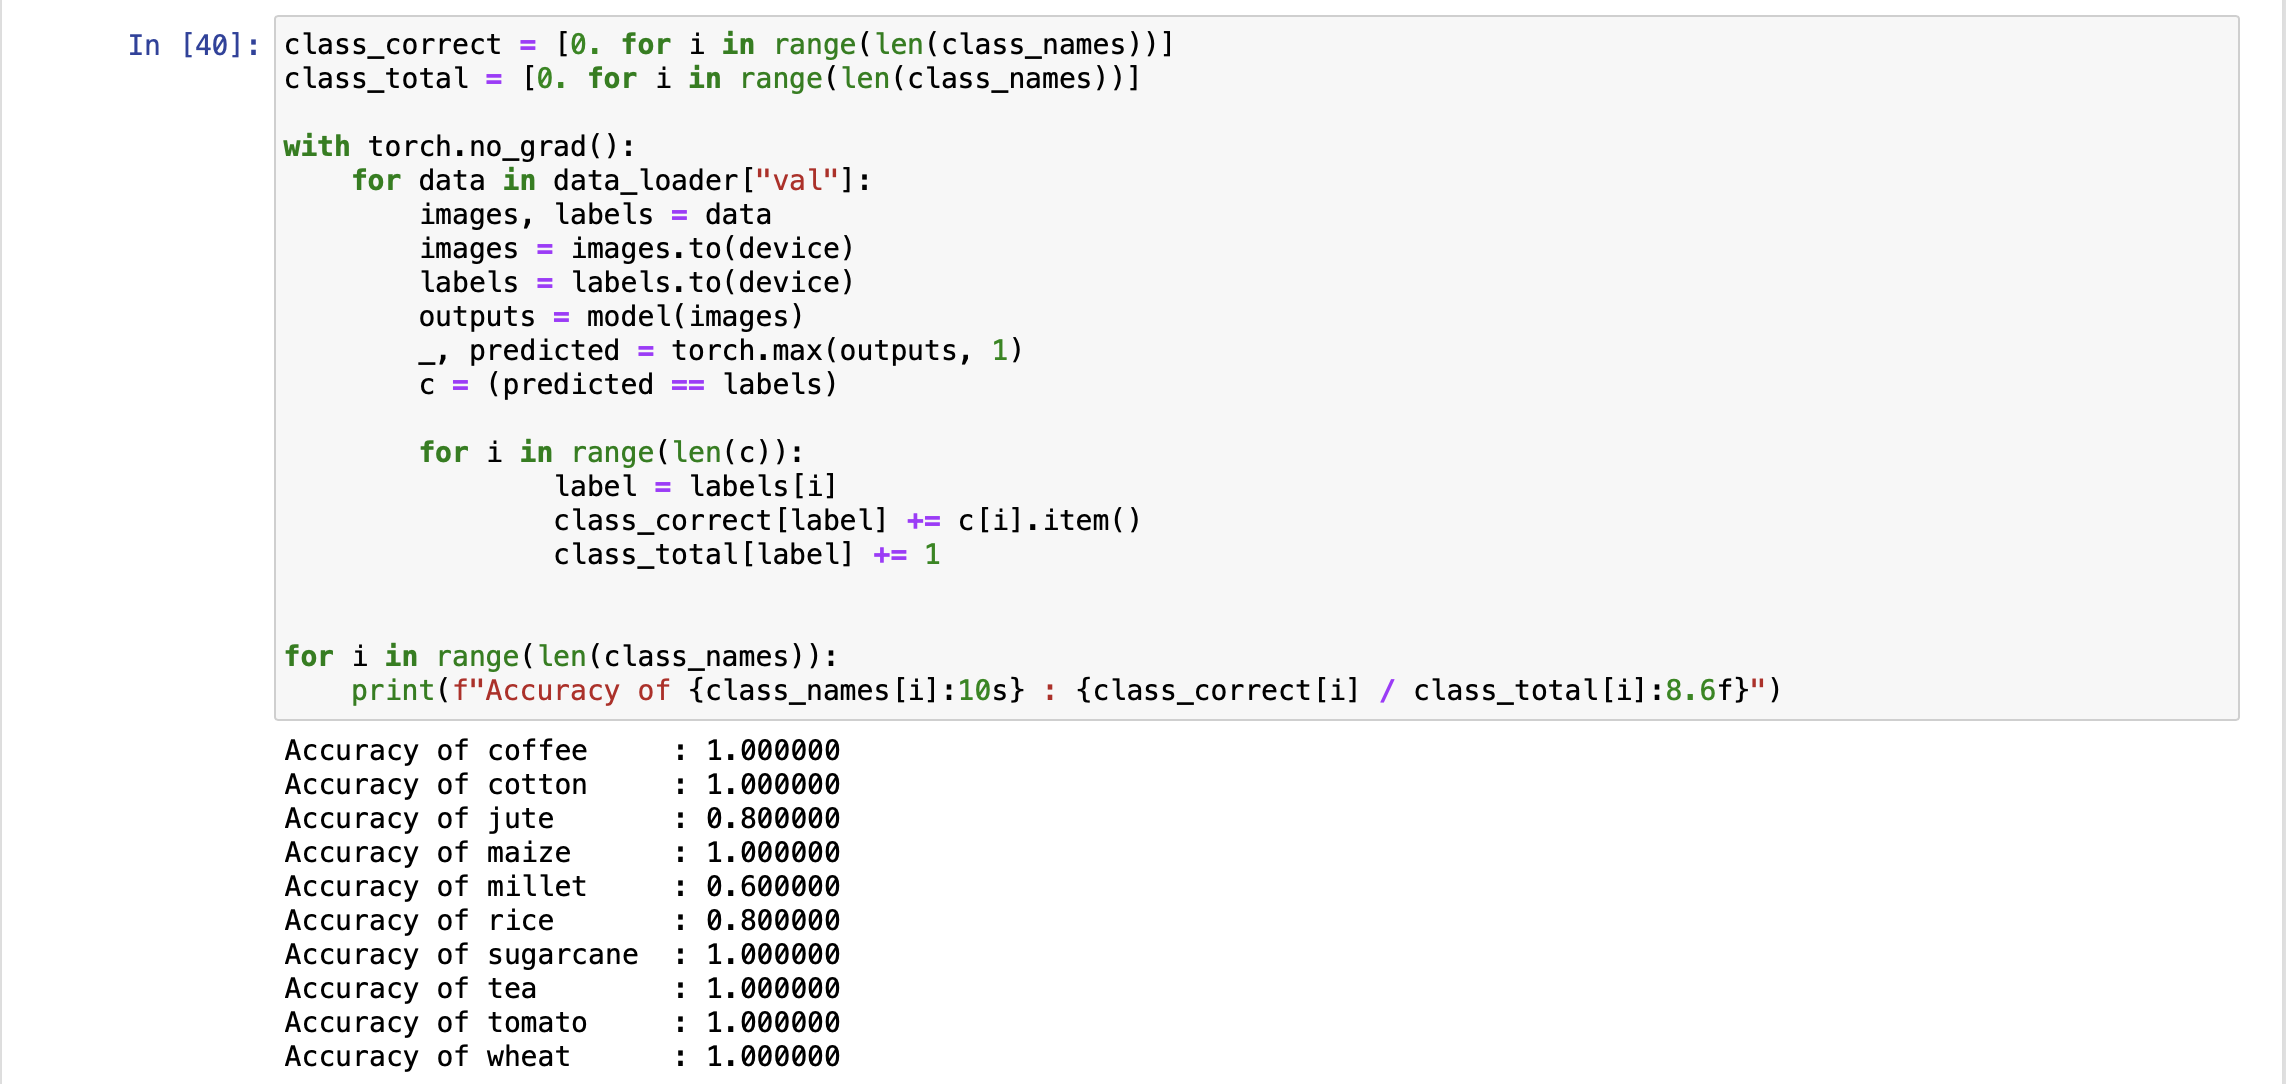
\includegraphics[width=\linewidth]{images/crop_class_acc.png}
  \caption{Crop Detection Class-wise Accuracy}
  \label{fig:test_ai_crop_class_acc}
\end{figure}\par

Disease Detection AI model, is slightly better due to the larger dataset size, with an accuracy of 94.8\%
\begin{figure}[H]
  \centering
  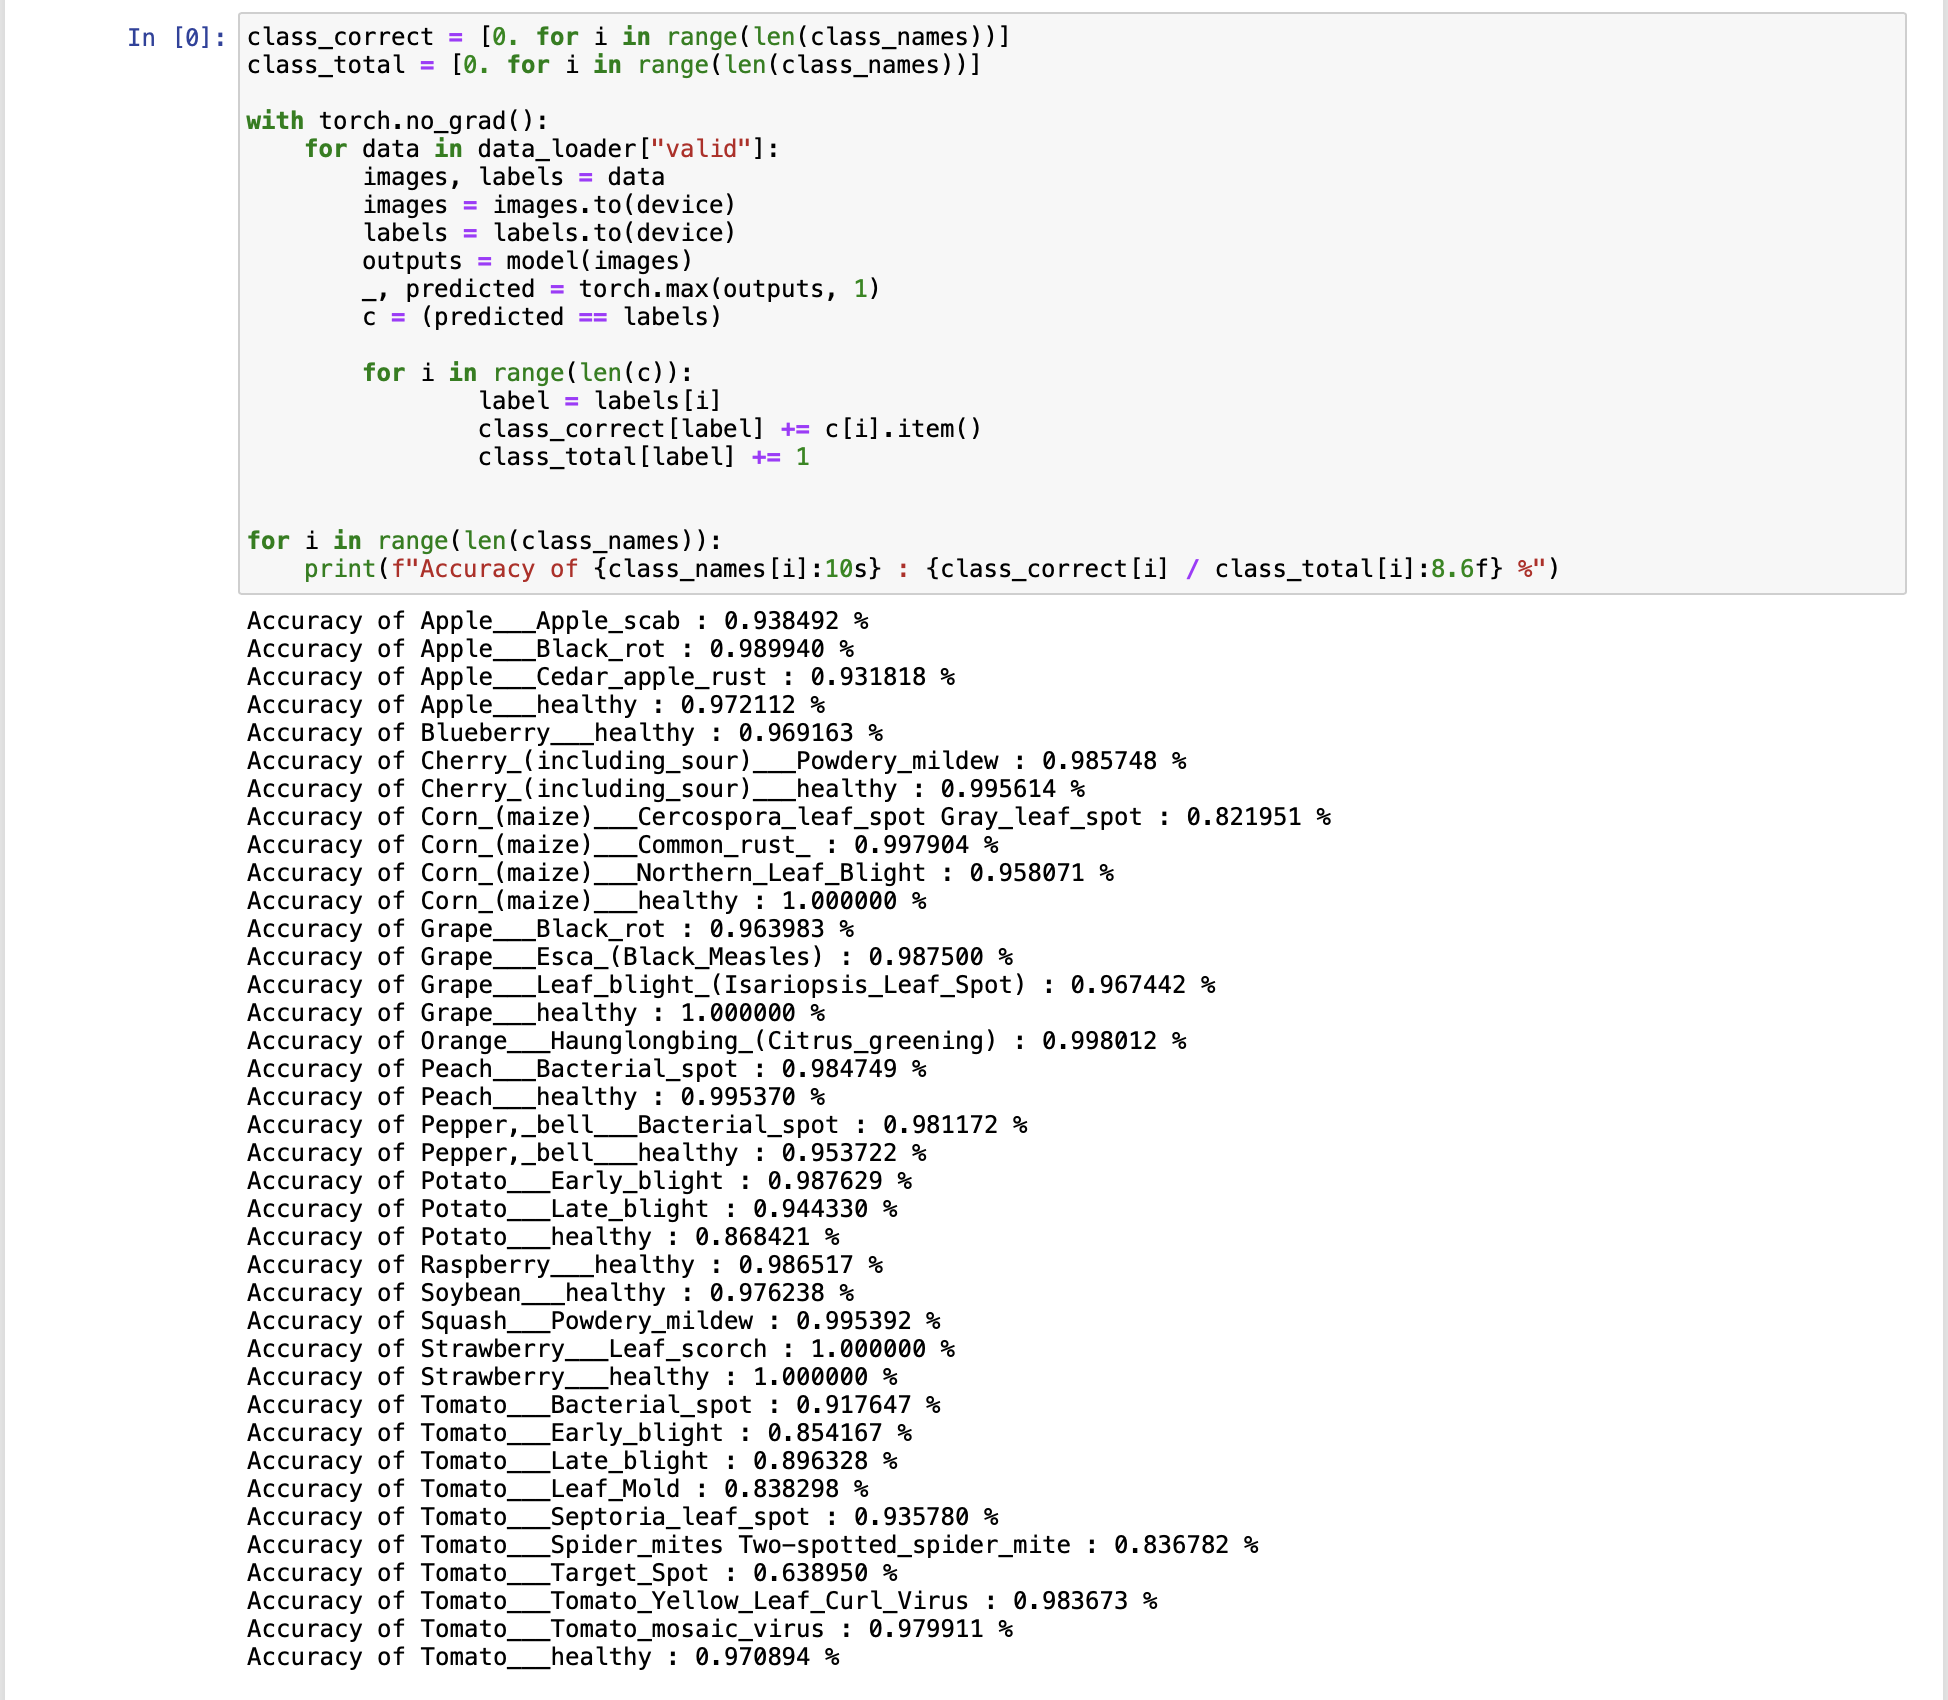
\includegraphics[width=\linewidth]{images/disease_class_acc.png}
  \caption{Crop Disease Detection Class-wise Accuracy}
  \label{fig:test_ai_disease_class_acc}
\end{figure}\par

\subsection{Testing Inference Server}

Testing of Inference Server is done using a tool called \textit{``Postman''}. Postman is an application that can be used for making HTTP 
requests like HTTP GET, POST, CREATE, PUT, DELETE. This tool also has an option to send multiple requests to test APIs.\par

For testing, the inference server, is run on local machine and Postman is used to send a POST request with image and compare the JSON 
responses with expected responses.\par

Following are some screenshots of automated API tests.\par

\begin{figure}[H]
  \centering
  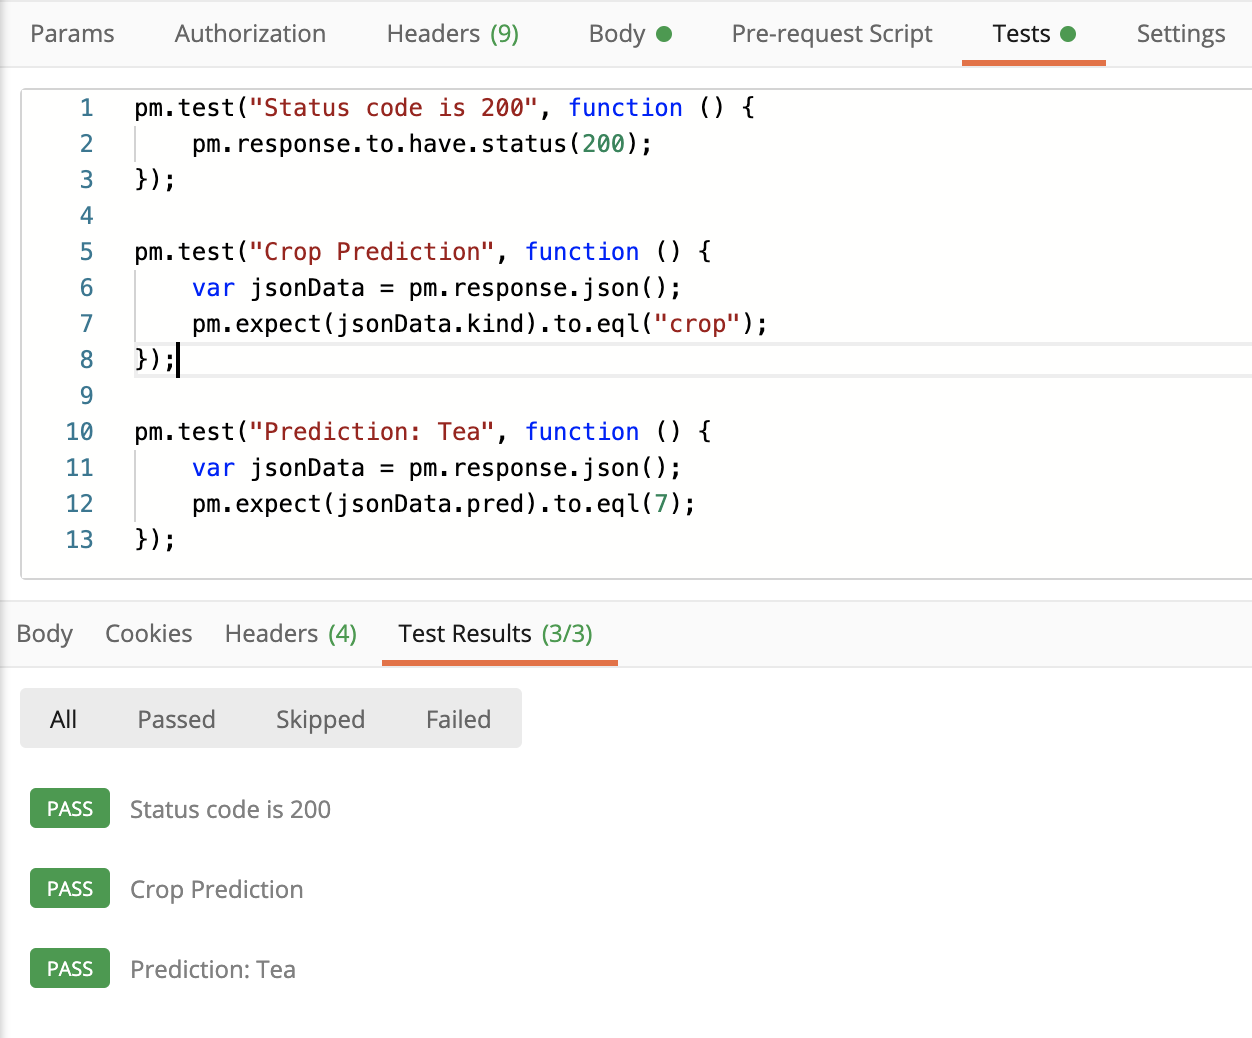
\includegraphics[width=0.7\linewidth]{images/api_crop.png}
  \caption{Test for Crop Detection API}
  \label{fig:test_api_crop}
\end{figure}
\begin{figure}[H]
  \centering
  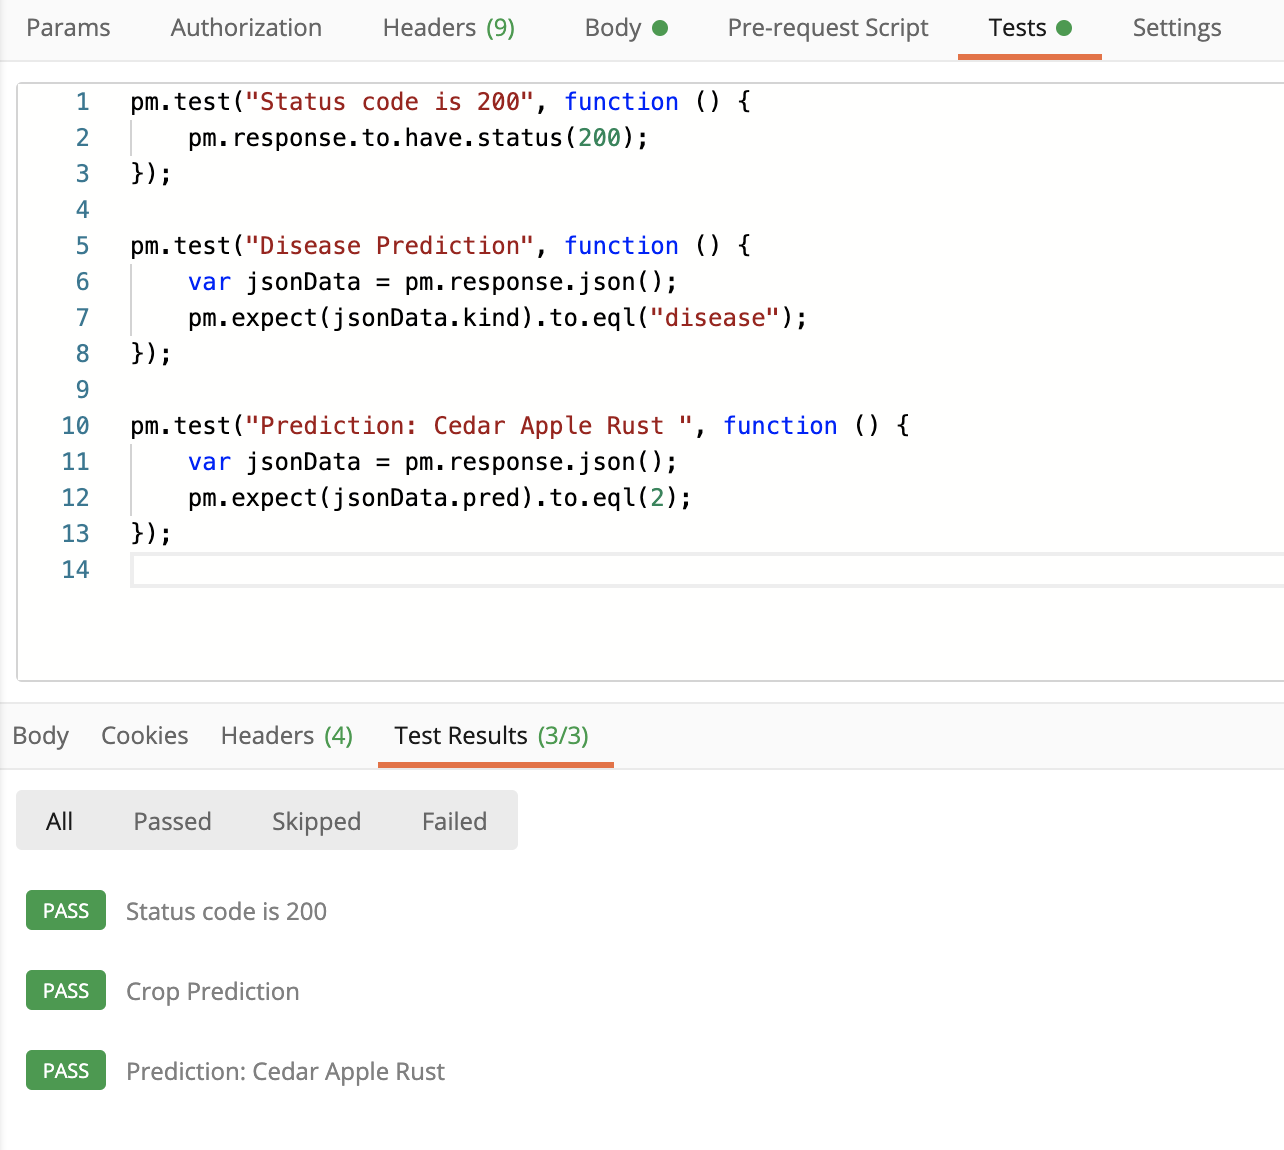
\includegraphics[width=0.7\linewidth]{images/api_disease.png}
  \caption{Test for Crop Disease Detection API}
  \label{fig:test_api_disease}
\end{figure}

\section{Mobile App Screenshots}
\begin{figure}[H]
    \centering
    \begin{minipage}{.5\textwidth}
      \centering
      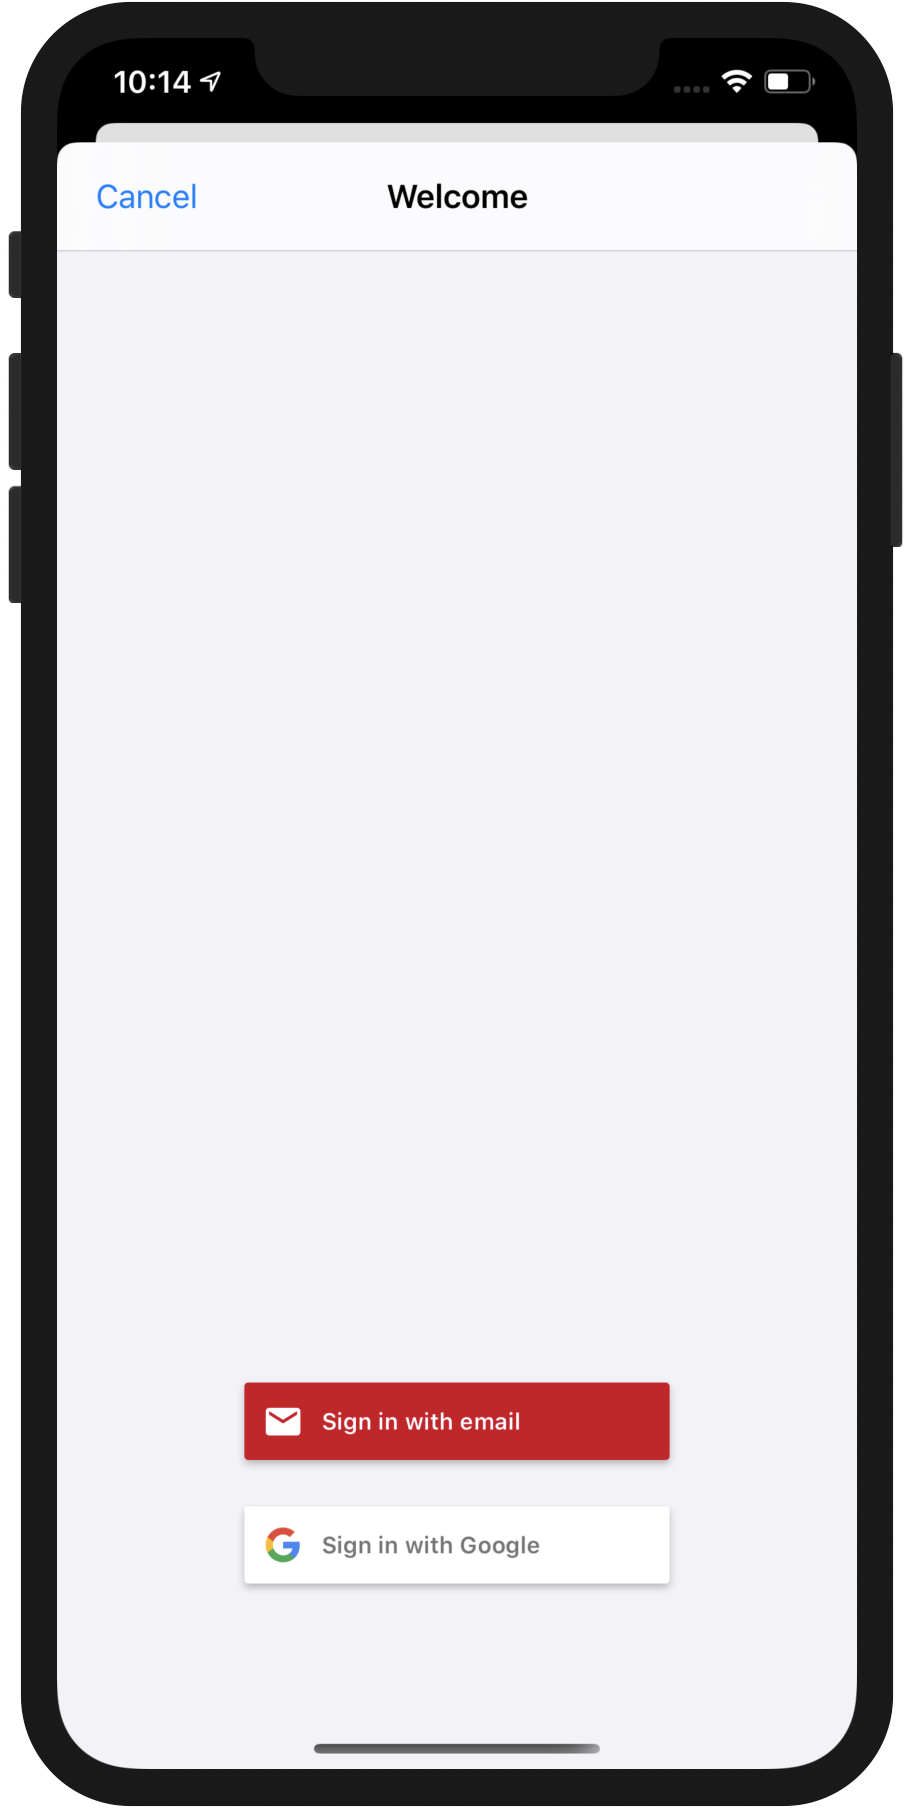
\includegraphics[width=5cm]{images/user_login.png}
      \captionof{figure}{User Login}
      \label{fig:ss_user_login}
    \end{minipage}%
    \begin{minipage}{.5\textwidth}
      \centering
      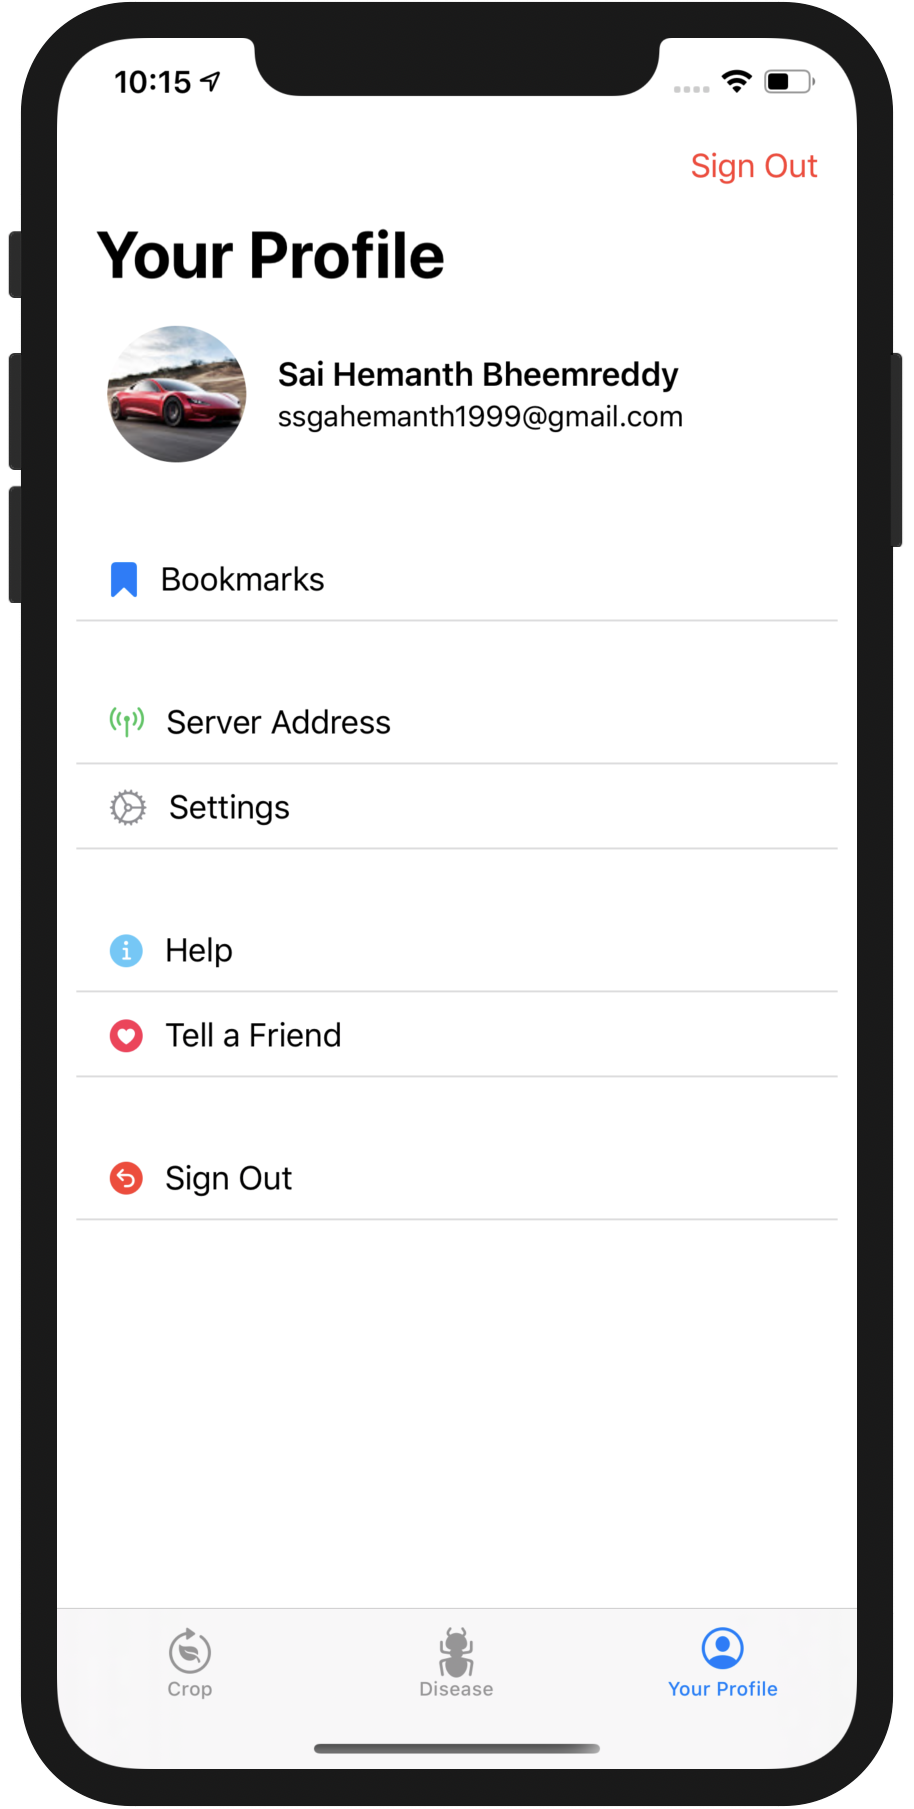
\includegraphics[width=5cm]{images/profile.png}
      \captionof{figure}{User Profile Tab}
      \label{fig:ss_user_profile}
    \end{minipage}
\end{figure}

\noindent When the user first launches the app, the user is asked to login.

\begin{figure}[H]
    \centering
    \begin{minipage}{.5\textwidth}
      \centering
      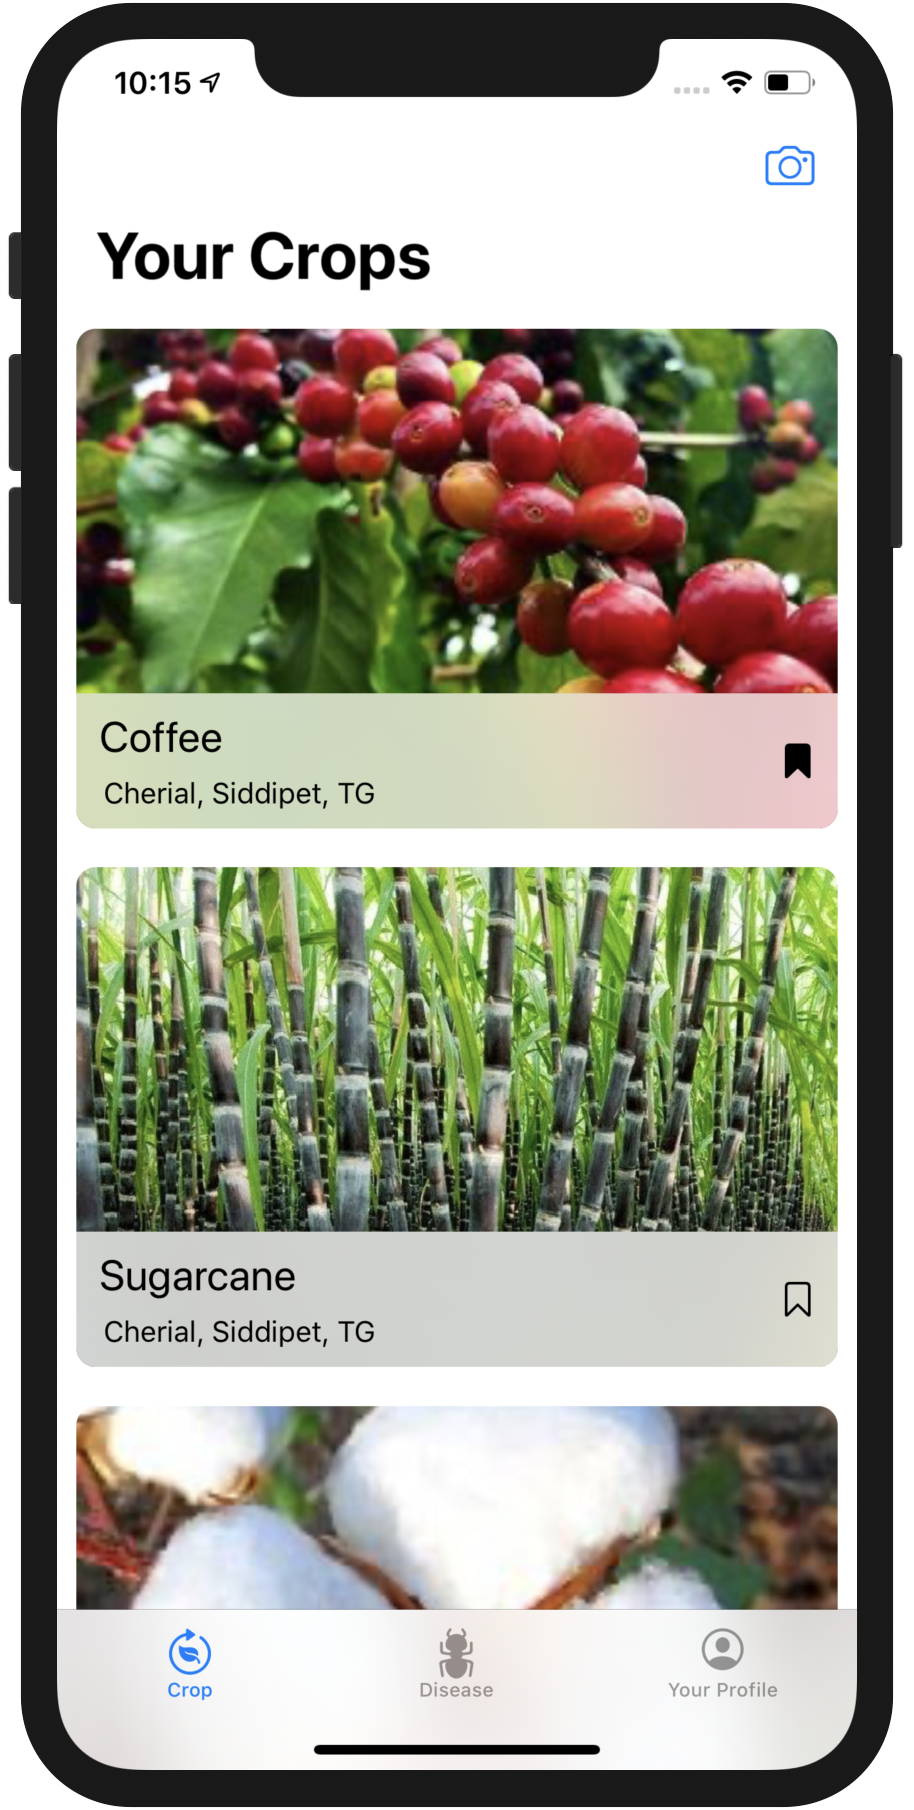
\includegraphics[width=5cm]{images/crop.png}
      \captionof{figure}{Crops Tab}
      \label{fig:ss_crop}
    \end{minipage}%
    \begin{minipage}{.5\textwidth}
      \centering
      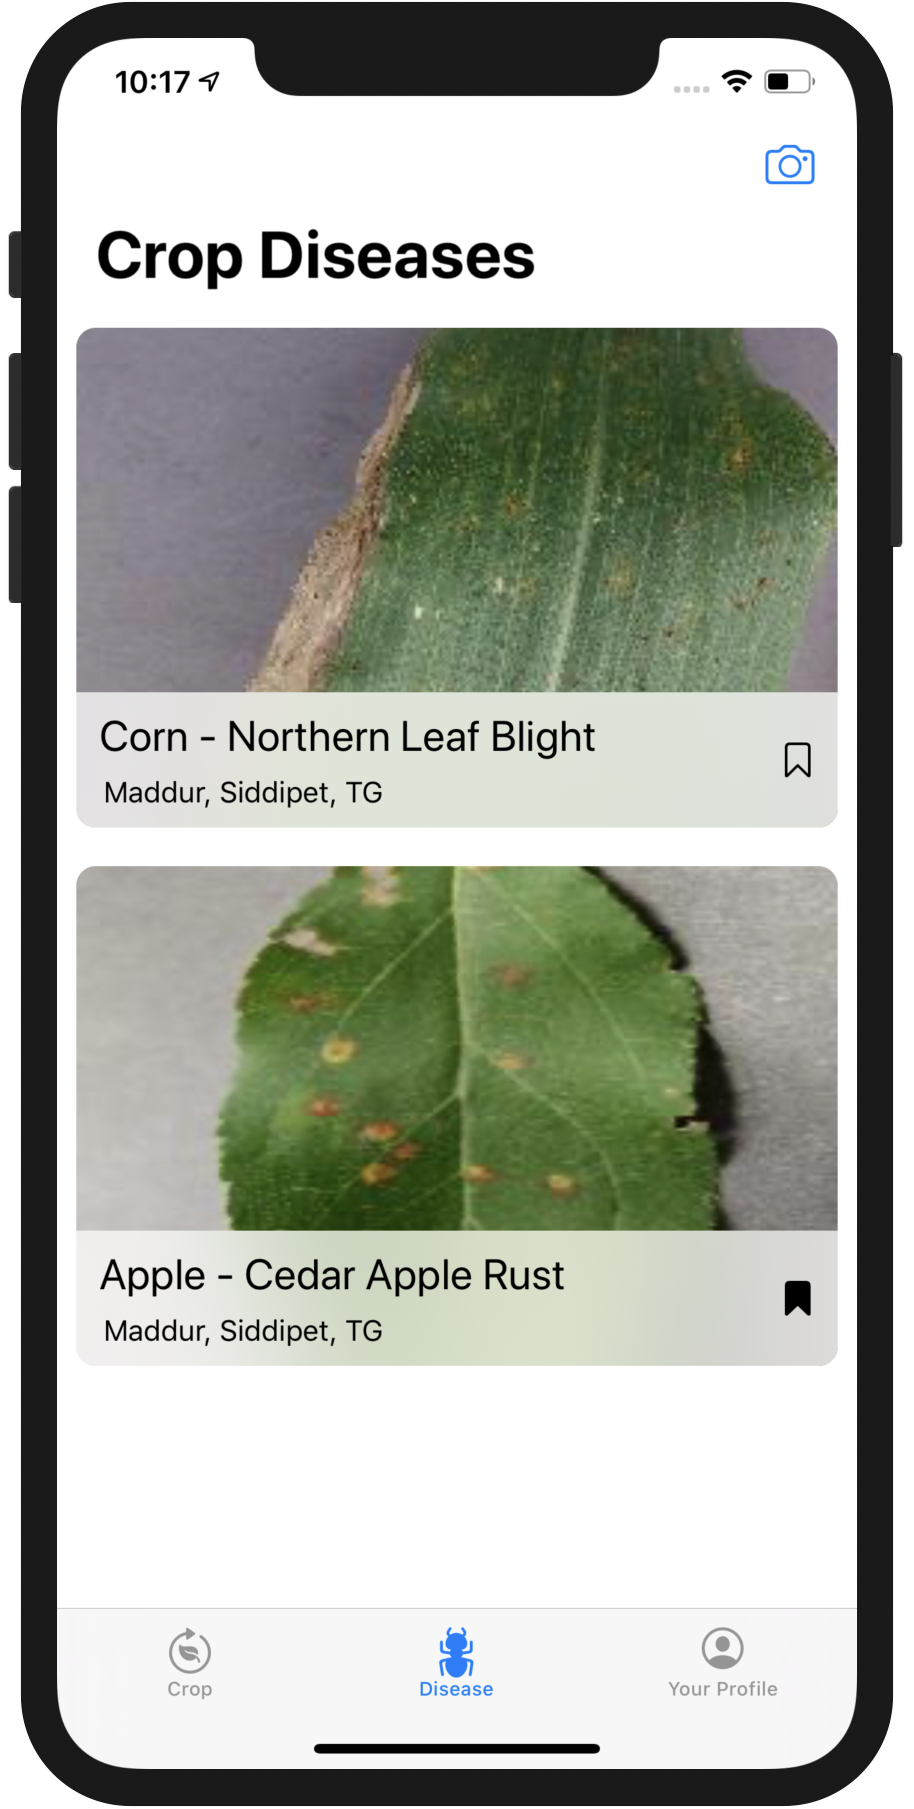
\includegraphics[width=5cm]{images/disease.png}
      \captionof{figure}{Crop Disease Tab}
      \label{fig:ss_disease}
    \end{minipage}
\end{figure}

\noindent These tabs show user's crops and all the information is available within single tap.

\begin{figure}[H]%
    \centering
    \subfloat{{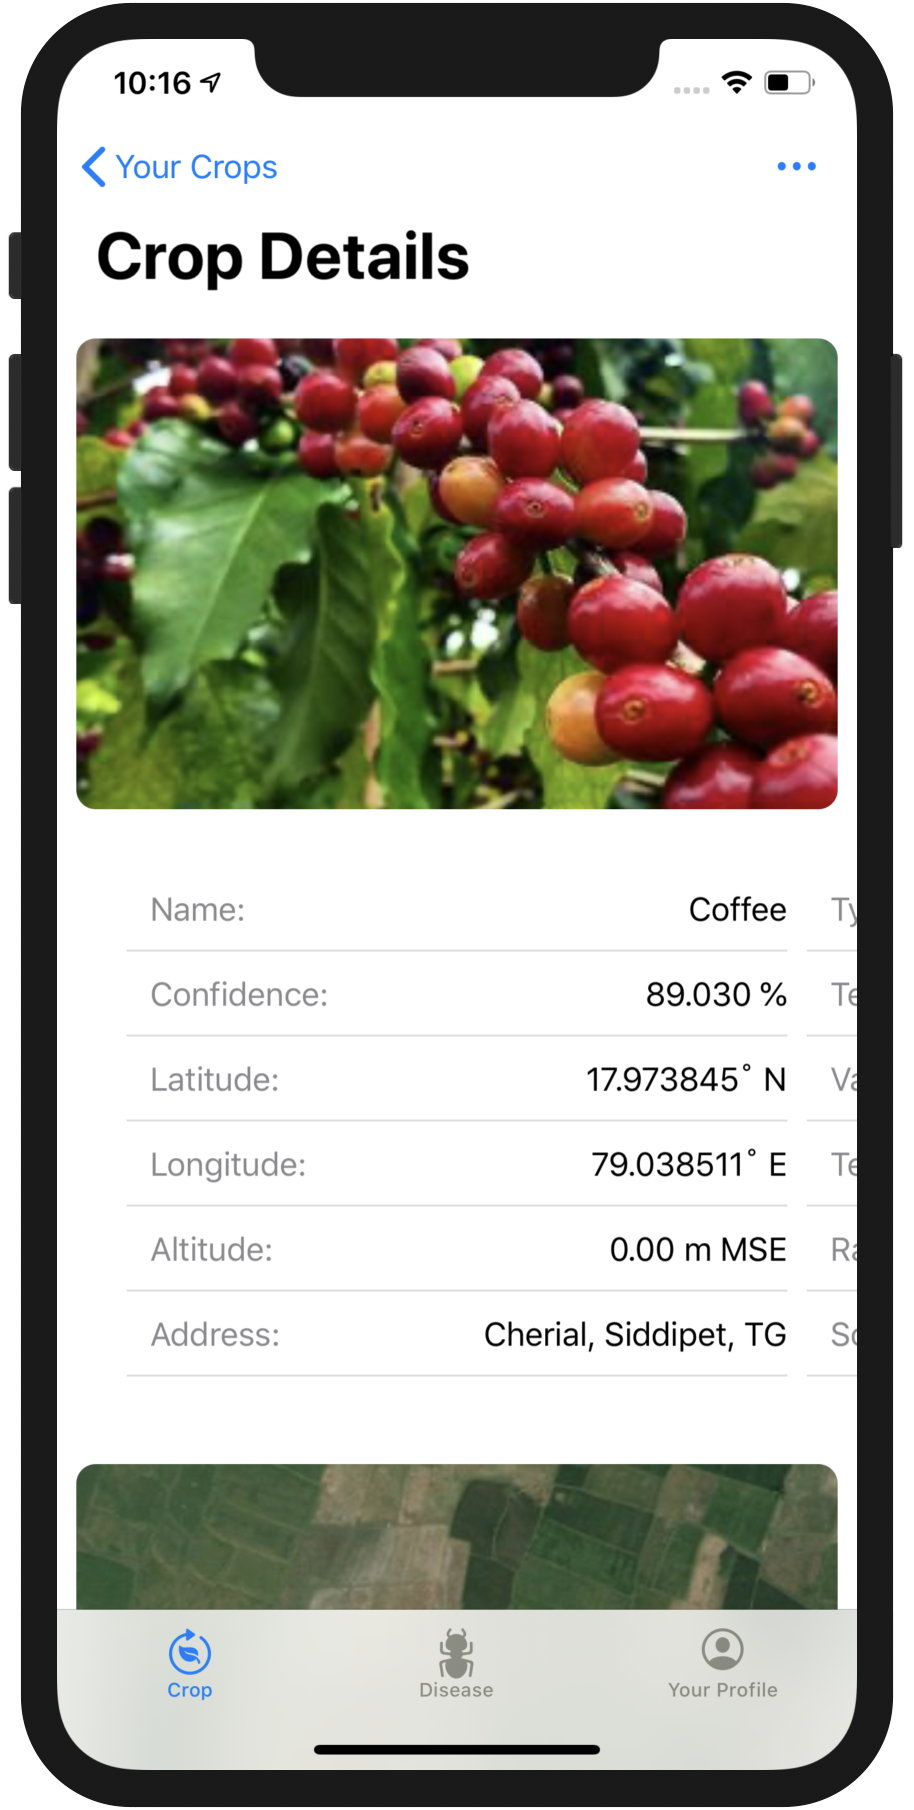
\includegraphics[width=5cm]{images/crop_details_1.png}}}%
    \qquad
    \subfloat{{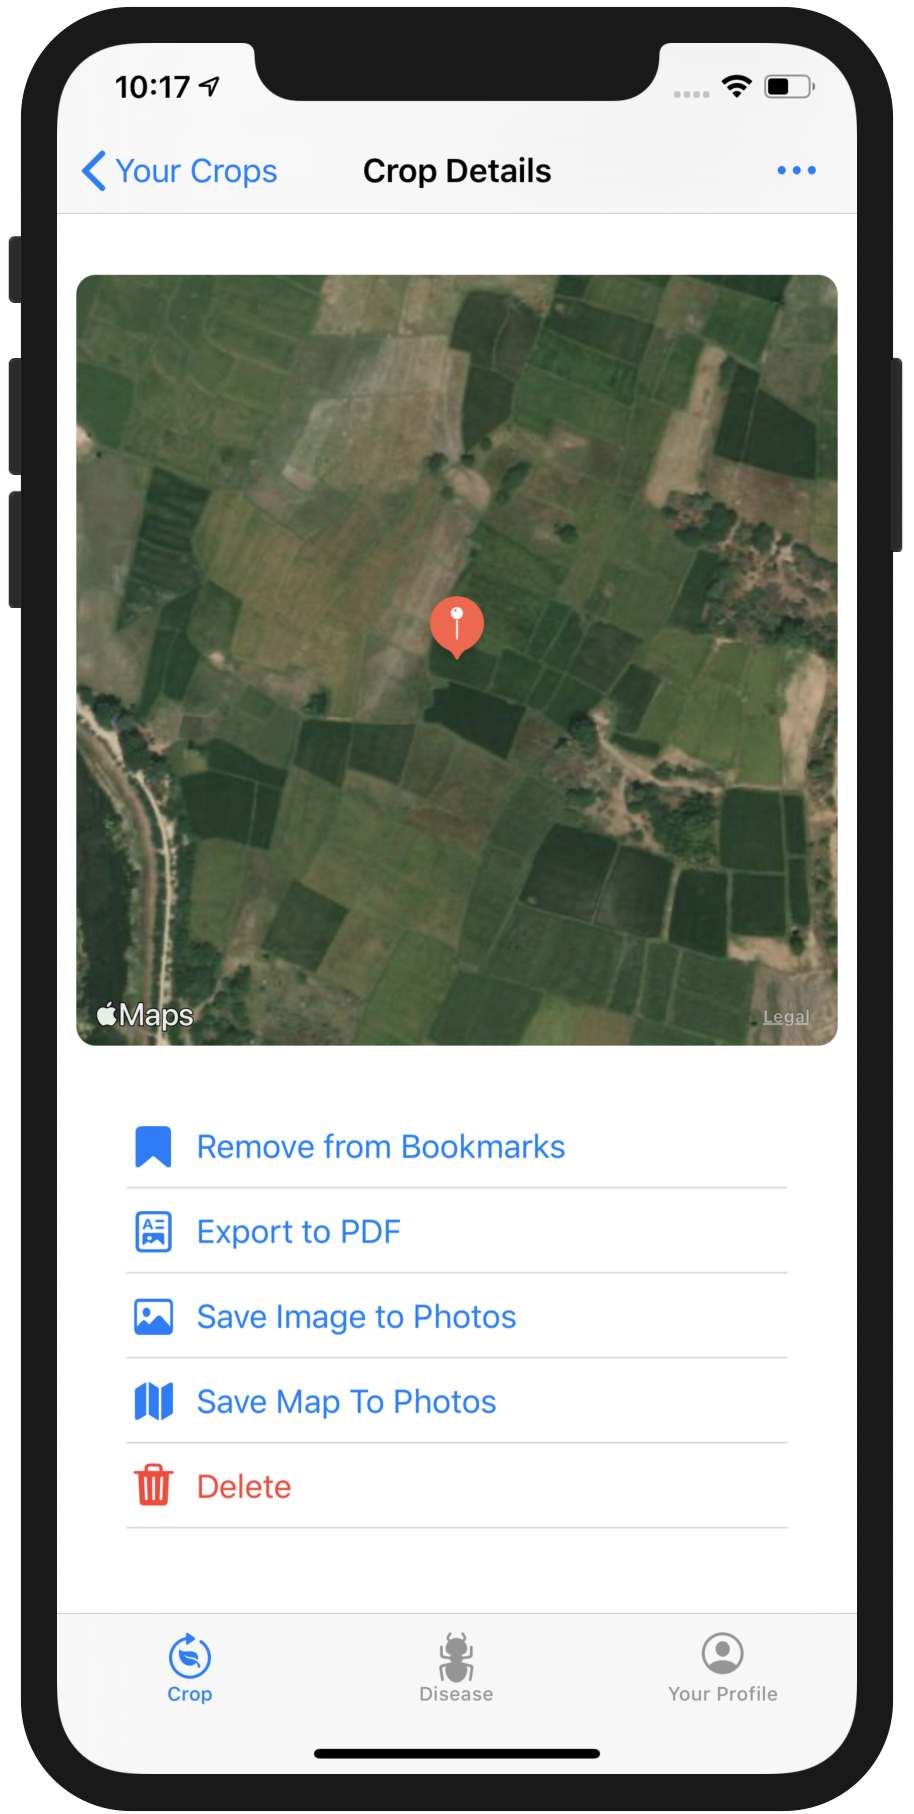
\includegraphics[width=5cm]{images/crop_details_2.png}}}%
    \caption{Crop Details Screen}
    \label{fig:ss_crop_details}%
\end{figure}

\noindent User can tap on any of the card in crop tab to get more details about his crops.

\begin{figure}[H]
    \centering
    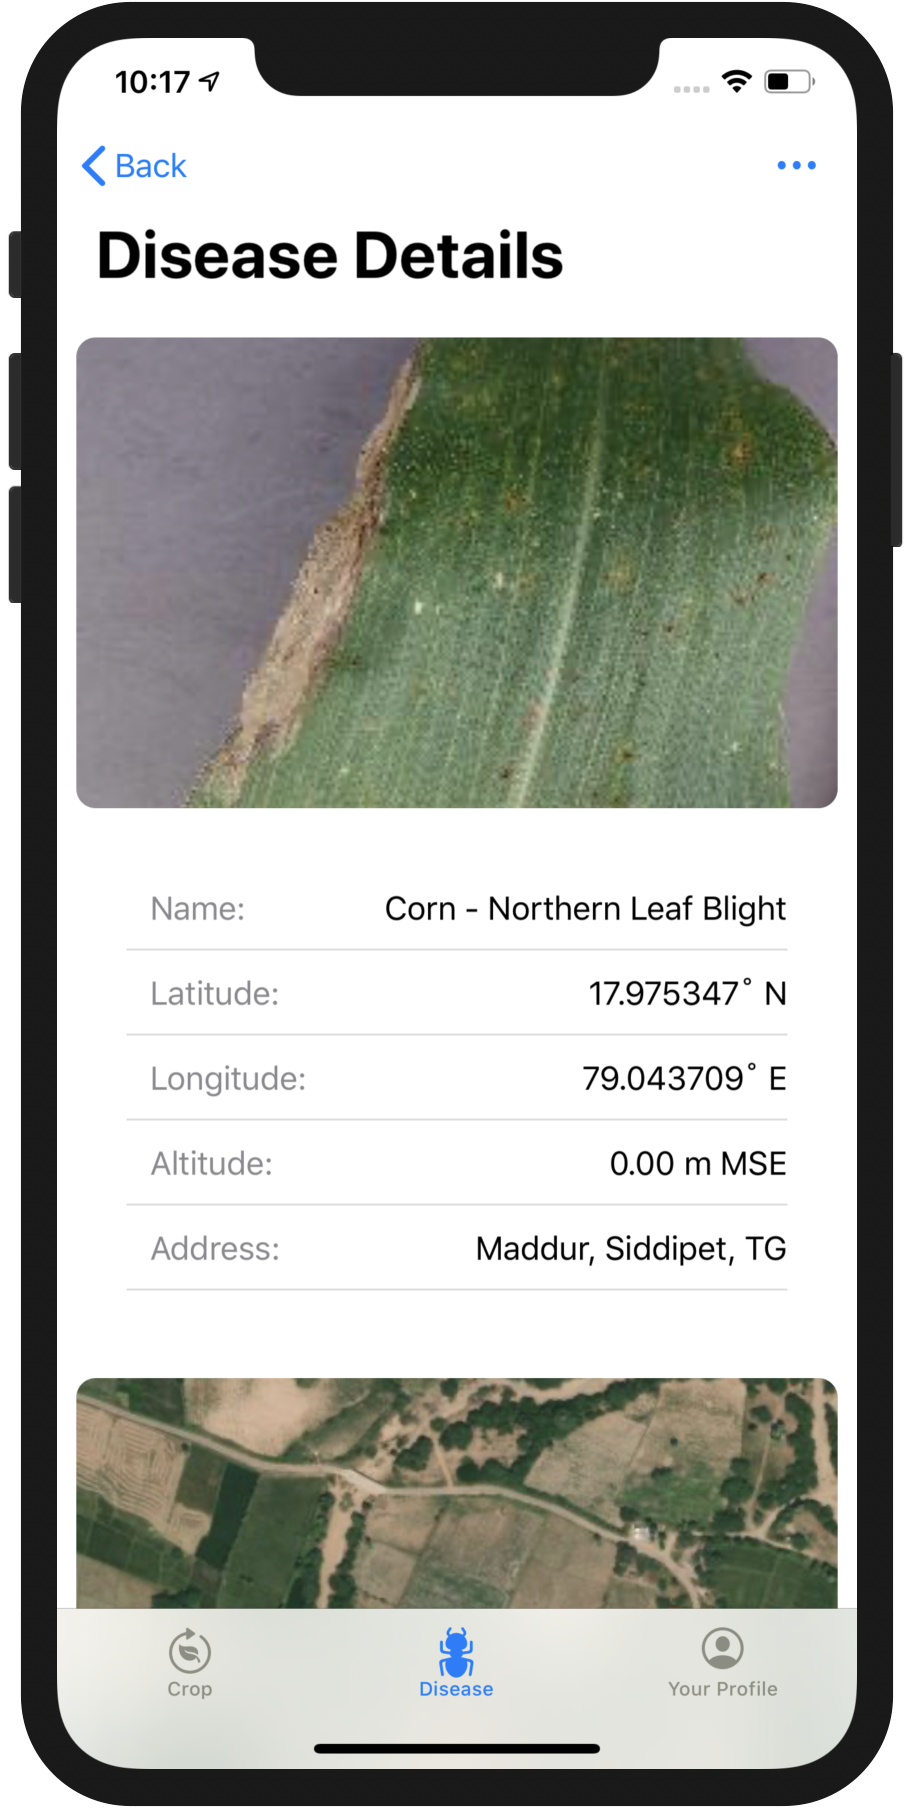
\includegraphics[width=5cm]{images/disease_details.png}
    \caption{Crop Disease Screen}
    \label{fig:ss_disease_details}
\end{figure}

\noindent User can tap on any of the card in disease tab to get more details about his crop disease.

\begin{figure}[H]
    \centering
    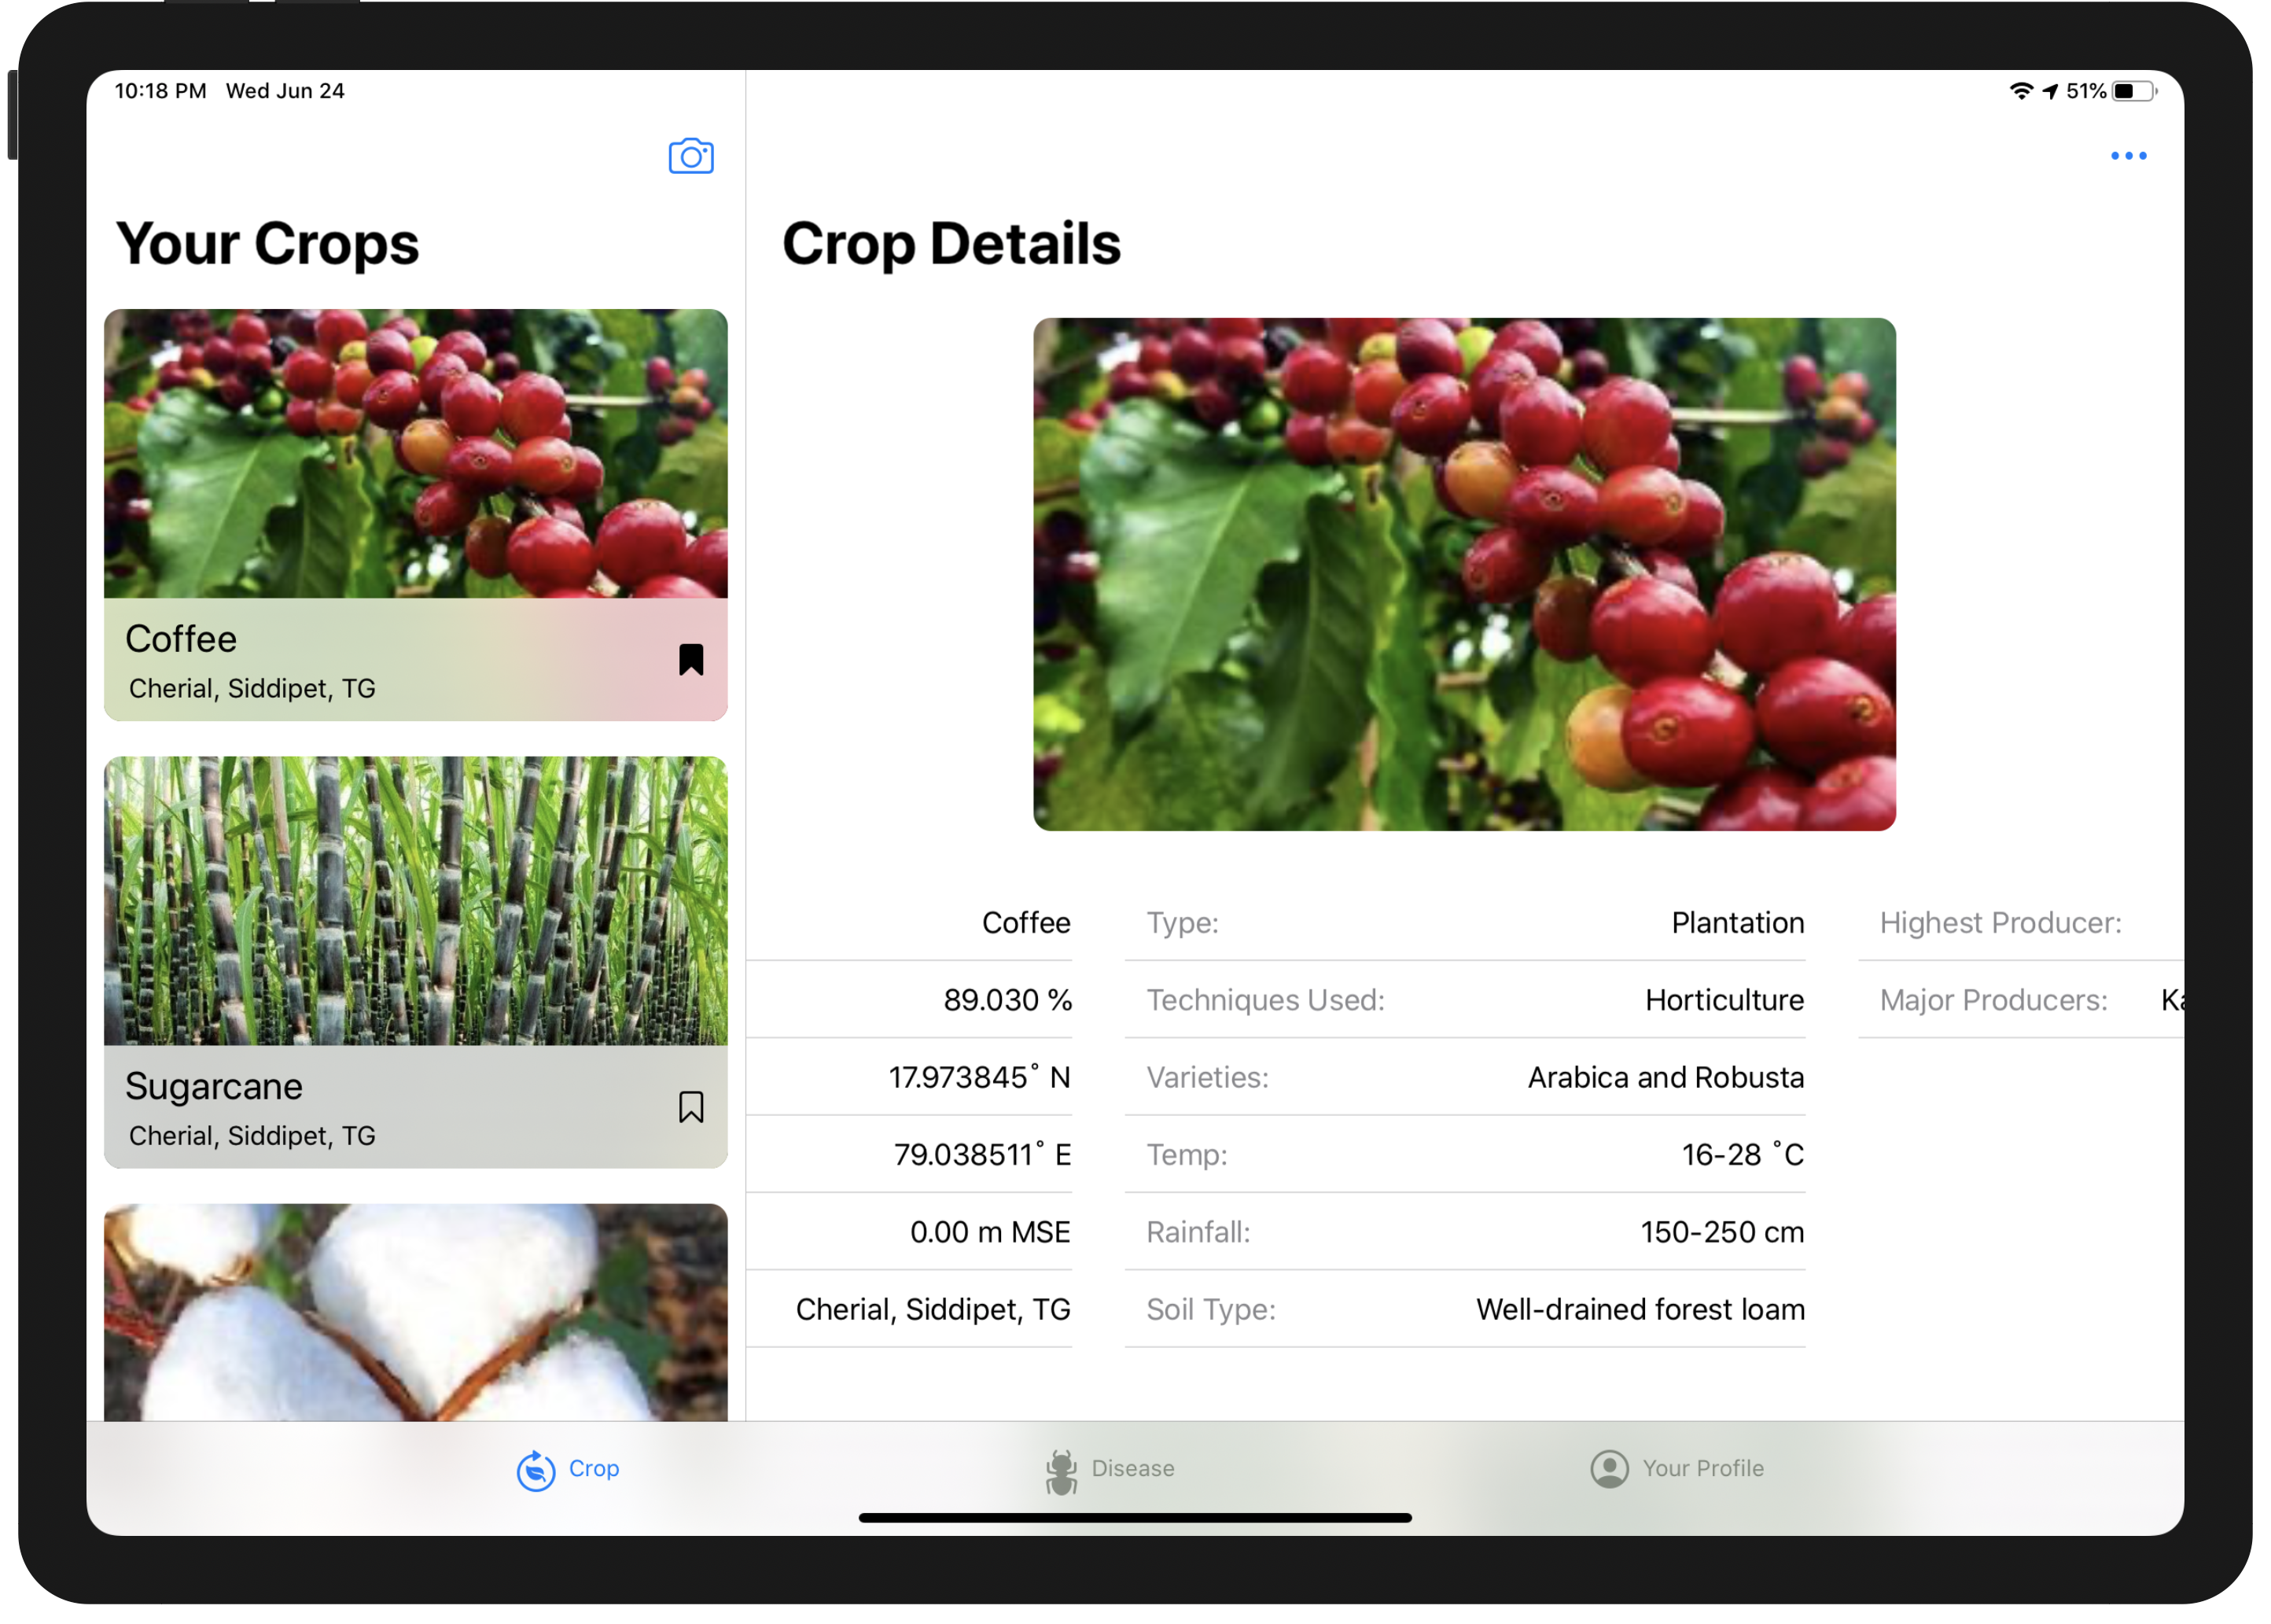
\includegraphics[width=0.75\linewidth]{images/ipad.png}
    \caption{Dynamic UI}
    \label{fig:ss_ipad}
\end{figure}

\noindent The app is made to run on any device and automatically adapts the UI to optimize the screen real estate.

\end{document}